\documentclass{article}
\usepackage{tabularx,fullpage,url}
\usepackage[top=1in, bottom=1in, left=.5in, right=.75in]{geometry}
\usepackage{amsmath,amssymb,graphicx,amsthm,xparse, color, mathrsfs} 
\usepackage{ epstopdf, fullpage}

\usepackage[ruled,vlined]{algorithm2e}
\usepackage{xifthen}
\usepackage{wrapfig}

\newcommand{\mypagebreak}{\begin{center}
		\noindent\makebox[\linewidth]{\rule{7.5in}{1pt}}
	\end{center}}


\newcommand{\bE}{\mathbb E}
\newcommand{\mS}{\mathcal S}

\newcommand{\showpoints}[1]{\textbf{(#1)}}


\begin{document}
{\Large\textbf{CSE 353: Homework 1 \hfill
Due Wednesday September 7}}


\mypagebreak

\begin{enumerate}

\item \showpoints{3 pts, 1 pt each} \emph{Machine learning fundamentals.}
Decide if the following ways of thinking fall under the umbrella of \emph{supervised}, \emph{semi-supervised}, or \emph{unsupervised} learning. Justify your answer. 

There is only and exactly one correct answer (no ``both" or ``all 3", no ``none"). 

\begin{tabular}{lcl}
\begin{minipage}{.6\textwidth}
\begin{enumerate}
\item I have just arrived to Middle Earth, and I am shocked by all the different creatures I see. Some are tall, some are short. Some have thorny heads, others have hair, or are bald. I decide to group everything I see into categories, and give them funny names (entpeople, olephants, etc.) These names are entirely my design, and capture feature similarities between clusters of species.




\item I have now met an ``entperson", who tells me that there are specific anatomical features that are unique to entmen and entwomen. For example, entmen tend to have really thorny heads, while entwomen have bushier feet. These are not hard and fast rules, in that there are entmen with bushy feat and entwomen with thorny heads, but they are rare. I therefore devise a classification scheme that decides the gender of entpeople based on these features. My entfriend then goes through a list of all the people in our neighborhood and helps me label them as men or women. I use this data to devise and refine a model, which I then take to the wild to do further inference.



\item I have now lived in Middle Earth for 150 years, so I have a pretty good grasp of the ``main'' species, such as dwarfs, or giants, or elves. But every once in a while I see something with completely new features, and am not sure exactly which of these categories it belongs. So, I use a mixture of the clustering strategy I used when I first arrived to kind of lump this new species in some category, and then use the labels I acquired by talking to a lot of different species over the past 150 years, and guess an appropriate species name for this new entity.



\end{enumerate}
\end{minipage}
&$\quad$&
\begin{minipage}{.3\textwidth}
\begin{center}
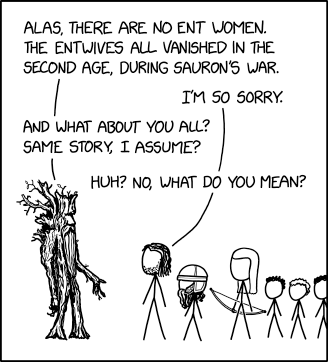
\includegraphics[width=\linewidth]{figs/entwives.png}\\
(credit: xkcd.com)
\end{center}
\end{minipage}
\end{tabular}





\item \showpoints{2 pts, 0.5 pts each} \emph{Independent or not independent.}
Two random variables $A$ and $B$ are \emph{independent} if, given distributions $p_A$ and $p_B$, we have 
\[
p_{A,B}(a,b) = p_A(a)p_B(b)
\]
where $p_{A,B}$ is their joint distribution.

In the following scenarios, decide if $A$ and $B$ are independent. Justify your answer.

\begin{enumerate}
\item $A$ and $B$ are discrete random variables and have the following p.m.f.s
\[
p_A(a) = \begin{cases}
0.25, & a = \text{red}\\
0.25, & a = \text{blue}\\
0.5, & a = \text{green}\\
\end{cases},
\qquad
p_B(b) = \begin{cases}
0.3, & b = \text{hat}\\
0.3, & b = \text{T-shirt}\\
0.2, & b = \text{skirt}\\
0.2, & b = \text{shoes}\\
\end{cases}
\]
and $p_{A,B}(a,b)$ are defined by the table below
\begin{center}
\begin{tabular}{l|ccc}
 & a = red & a = blue & a = green\\\hline
b = hat& 0.075 & 0.075 & 0.15\\
b = T-shirt& 0.075 & 0.075 & 0.15\\
b = skirt&0.05 & 0.05 & 0.1\\
b = shoes&0.05 & 0.05 & 0.1\\
\end{tabular} 
\end{center}



\item $A$ and $B$ are uniform distributions, where 
\[
f_A(a) = \begin{cases} 1 & -1 \leq a \leq 0 \\ 0 & \text{else,}
\end{cases}
\qquad
f_B(b) = \begin{cases} 1 & 0 \leq b \leq 1 \\ 0 & \text{else,}
\end{cases}, 
\qquad
f_{A,B}(a,b) = \begin{cases} 4/3 &  |a+b| \leq 1/2 \\ 0 & \text{else,}
\end{cases}
\]


\item $A$ follows the p.m.f.
\[
p_A(a) = \begin{cases}
0.5, & a = 1\\
0.5, & a = -1\\
\end{cases}
\]
and $B = A\cdot C$ where
\[
p_C(c) = \begin{cases}
0.9, & c = 1\\
0.1, & c = -1\\
\end{cases}
\]




\item $A$ and $B$ are Gaussian distributions, with   the following properties:
\[
\bE[A] = 0,\quad \bE[B] = 1, \quad\bE[A^2] = 1, \quad\bE[(B-1)^2] = 1/2, \quad\bE[A(B-1)] = -1.
\]
Writing in terms of the usual Gaussian distribution form, if we form a random vector as $X = \begin{bmatrix} A \\ B\end{bmatrix}$, then
\[
\mu = \begin{bmatrix} \bE[A]\\\bE[B]\end{bmatrix}, \qquad
\Sigma = \begin{bmatrix} \bE[(A-\bE[A])^2] & \bE[(A-\bE[A])(B-\bE[B])] \\\bE[(A-\bE[A])(B-\bE[B])] & \bE[(B-\bE[B])^2] \end{bmatrix} 
\]


\end{enumerate}






\item  \showpoints{5 pts}  \textbf{$K$-nearest neighbors classification.}  We will now try to use the KNN classifier to classify MNIST digits. 

\begin{itemize}
\item Open \texttt{hw1\_minst\_release.ipynb}. Load the necessary packages and the data, and take a look at how the data is formatted and structured. I have done all the ``data cleaning" needed for this assignment (which is very minimal for this exercise). I have also included a function \texttt{get\_small\_dataset} which will return a subset of the training data (60000 samples!) so that we can reasonably train some things on even the worst laptops. 

\item  \showpoints{2 pts}  \textbf{Distance function.} The first step in establishing a KNN classifier is deciding what is going to be your metric for ``distance", and writing a function that, given the training data \texttt{Xtrain} and query point \texttt{zquery}, can as efficiently as possible return a vector of distances between \texttt{zquery} and all of the datapoints in \texttt{Xtrain}. 

There are many ways to do this, some faster than others. In general, if your implementation involves a \texttt{for loop}, you may be in for a lot of waiting and some very warm laptops. One implementation that avoids \texttt{for loop}s is to really try to use the optimized numerical linear algebra functions of the numpy library as much as possible, e.g. using functions like \texttt{np.dot}, \texttt{np.sum}, etc. 

The distance function we will use is the 2 norm squared; specifically:
\[
d(x_i,z) = \sum_{j=1}^n (x_i[j]-z[j])^2.
\]
There are several different ways of implementing this in your code, some more efficient than others. (Hint: think about what you can preprocess.)

\textbf{In your writeup}, print what you see when you run the box, e.g. the print outputs of

\begin{verbatim}
print(get_dist(Xtrain,Xtrain[0,:])[0])
print(get_dist(Xtrain,Xtest[0,:])[10])
print(get_dist(Xtrain,Xtest[10,:])[50])
\end{verbatim}



\item  \showpoints{1 pts}  \textbf{Prediction.} Implement a $K$-nearest-neighbor classification predictor, which takes a test data point, finds the closest point (in terms of Euclidean distance) in the train data set, and returns the KNN prediction. Use a majority vote scheme to decide which label to return; use whatever scheme you wish to break ties. 

Hint: take a look at \texttt{scipy.stats.mode()}

\textbf{In your writeup}, print the  output for $K=3$ and $m = 100$, e.g. the output for the lines

\begin{verbatim}
print(ytest_pred[:20])
print(ytest[:20])
\end{verbatim}



\item \textbf{Evaluate based on classification accuracy.} Now write a function that returns the classification accuracy given a list of true labels (\texttt{ytrue}) and predicted labels (\texttt{ypred)}. 


\textbf{In your writeup}, print classification accuracy of the test set.


\item  \showpoints{2 pts}  \textbf{Hyperparameter tuning.}  I have included in the next box an experiment in which your KNN predictor is tested for a training dataset with 100, 1000, and 2500 data samples. In each case, the code will run your predictor and return three numbers: $m$, the prediction accuracy, and the prediction runtime. Run this box and \textbf{return the classification accuracy and runtimes} for $m = 100,1000,2500$ and $K = 1,3,5$.

\begin{center}
\begin{tabular}{cccc}
$m$ & $K$ & accuracy & runtime (sec)\\\hline
100 & 1 & & \\
100 & 3 & & \\
100 & 5 & & \\
1000 & 1 & & \\
1000 & 3 & & \\
1000 & 5 & & \\
2500 & 1 & & \\
2500 & 3 & & \\
2500 & 5 & & \\
\end{tabular}
\end{center}

 Comment a bit on the performance of the model for these different hyperparameter choices. In particular:

\begin{itemize}
\item Is it feasible to run this model for the full $m = 60000$ training dataset in runtime? Is it advisable?



\item How does the accuracy depend on $K$ for different values of $m$?






\end{itemize}


\end{itemize}



\end{enumerate}


\end{document}